\documentclass[12pt]{article}
\usepackage{amsmath}
\usepackage{fullpage}
\usepackage{graphicx}
\usepackage{subcaption}
\usepackage{alltt}
\author{
Niraj Mahajan \\
\texttt{180050069} \and
Raaghav Raaj \\
\texttt{180050082}}
\title{CS 215 - Assignment 2}


\begin{document}
\maketitle

\newpage
\section{Question 5}



\paragraph{Usage of MATLAB Code}
\begin{itemize}
\item Load code in the following path 'matlab\_code/Q5/q5.m'
\item Run the code
\item This should create two figures simultaneously (probably one on the other, you may have to separate them). They both will iterate over all N values and show the respective histograms and cdfs
\item After this, two more figures will be created. Both will have MAD plotted against N. But one will have it plotted in the usual way, but the other will have it plotted against semilogx, which will have better visibility.
\item All plots are inlcuded in this report, at the end, (after question 6).
\item I have also saved these plots in the directory 'matlab\_code/Q5/jpgs'
\end{itemize}

\begin{figure}[h!]
  \centering
  \begin{subfigure}[b]{0.4\linewidth}
    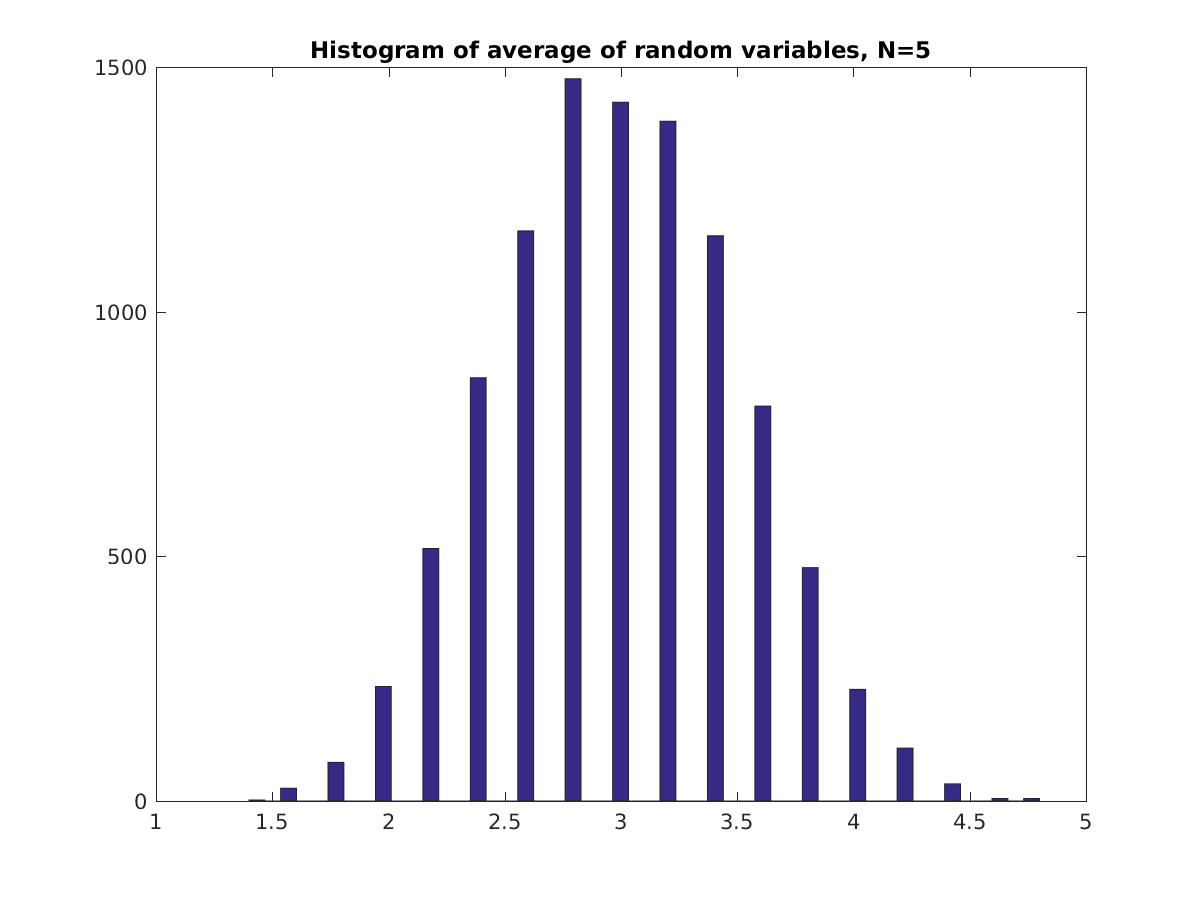
\includegraphics[width=\linewidth]{jpgs/histograms/5_hist.jpg}
    \caption{Histogram.}
  \end{subfigure}
  \begin{subfigure}[b]{0.4\linewidth}
    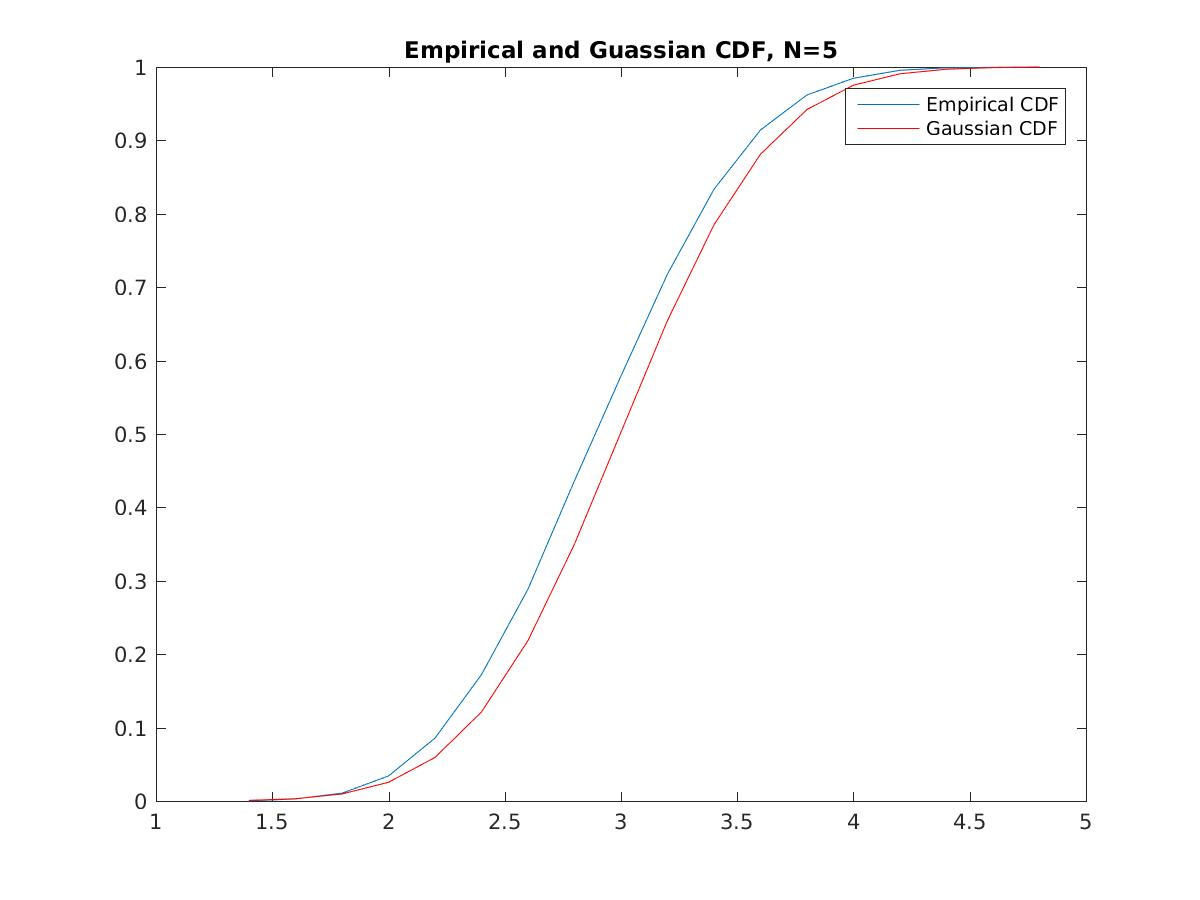
\includegraphics[width=\linewidth]{jpgs/cdfs/5_cdf.jpg}
    \caption{More Histogram.}
  \end{subfigure}
  \caption{N=5}
\end{figure}
\begin{figure}[h!]
  \centering
  \begin{subfigure}[b]{0.4\linewidth}
    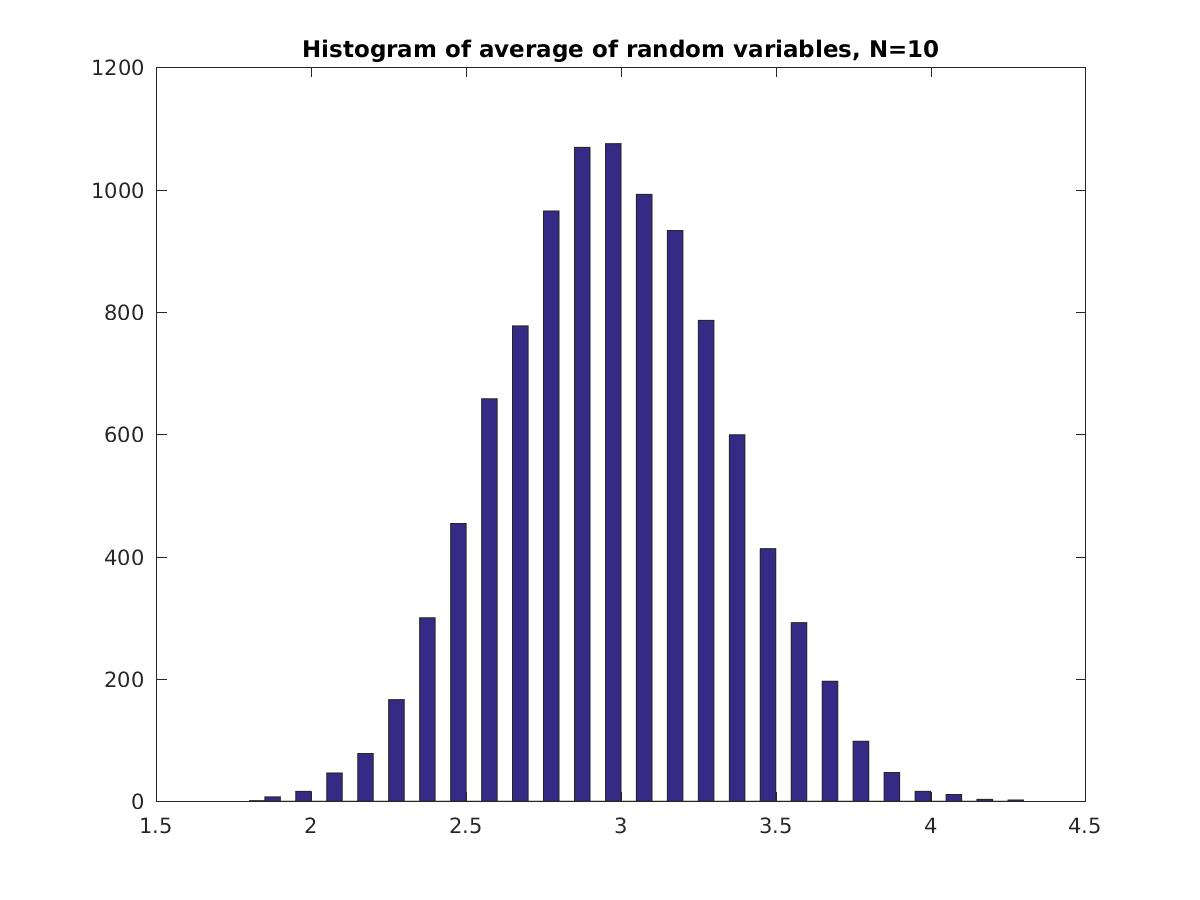
\includegraphics[width=\linewidth]{jpgs/histograms/10_hist.jpg}
    \caption{Histogram.}
  \end{subfigure}
  \begin{subfigure}[b]{0.4\linewidth}
    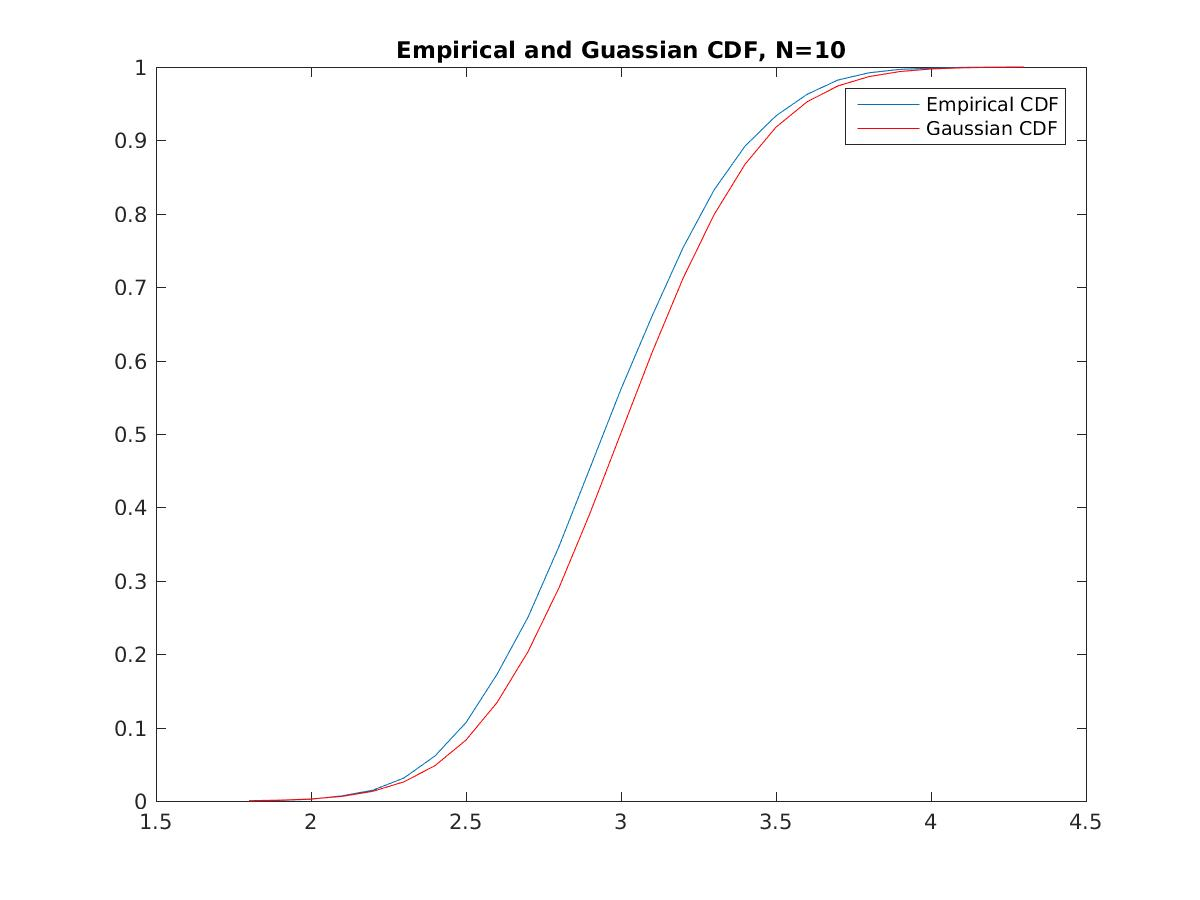
\includegraphics[width=\linewidth]{jpgs/cdfs/10_cdf.jpg}
    \caption{More Histogram.}
  \end{subfigure}
  \caption{N=10}
\end{figure}

\begin{figure}[h!]
  \centering
  \begin{subfigure}[b]{0.4\linewidth}
    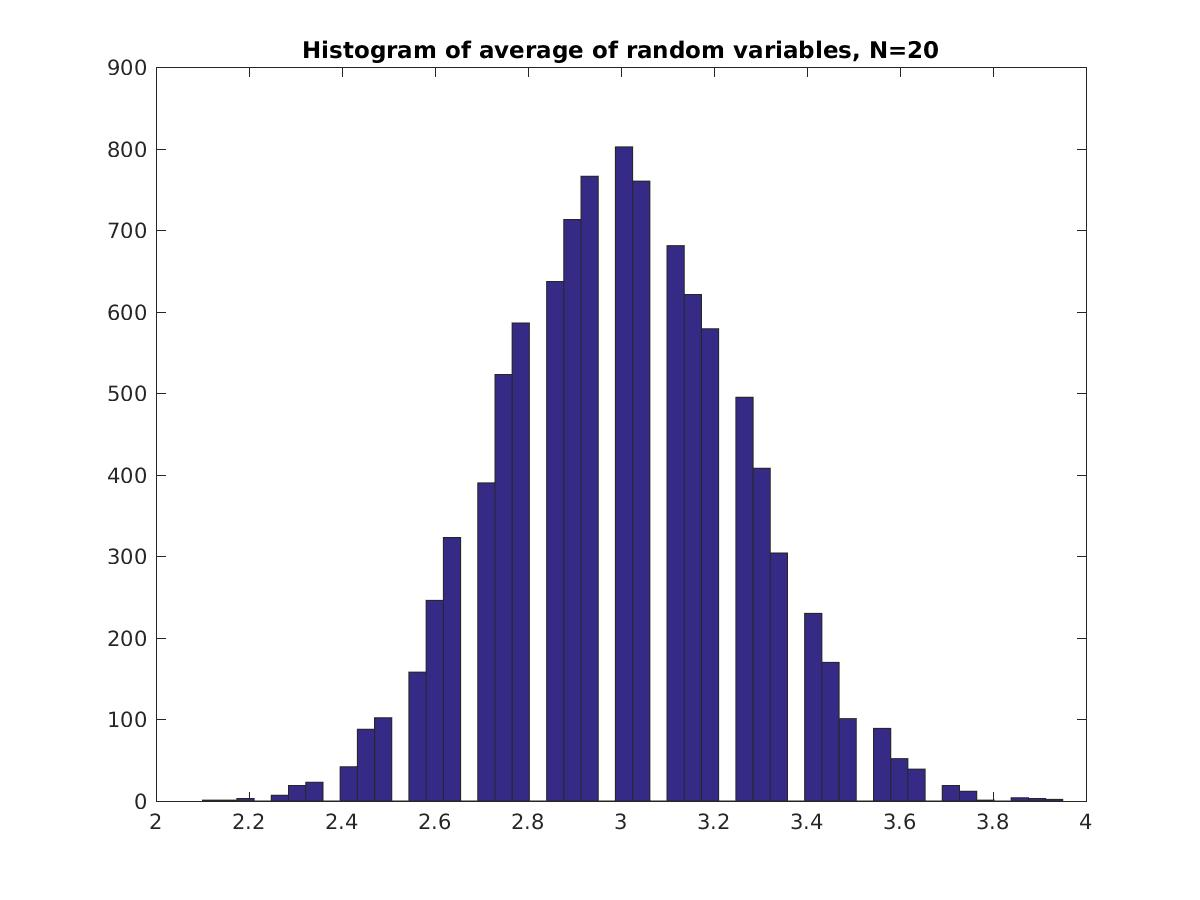
\includegraphics[width=\linewidth]{jpgs/histograms/20_hist.jpg}
    \caption{Histogram.}
  \end{subfigure}
  \begin{subfigure}[b]{0.4\linewidth}
    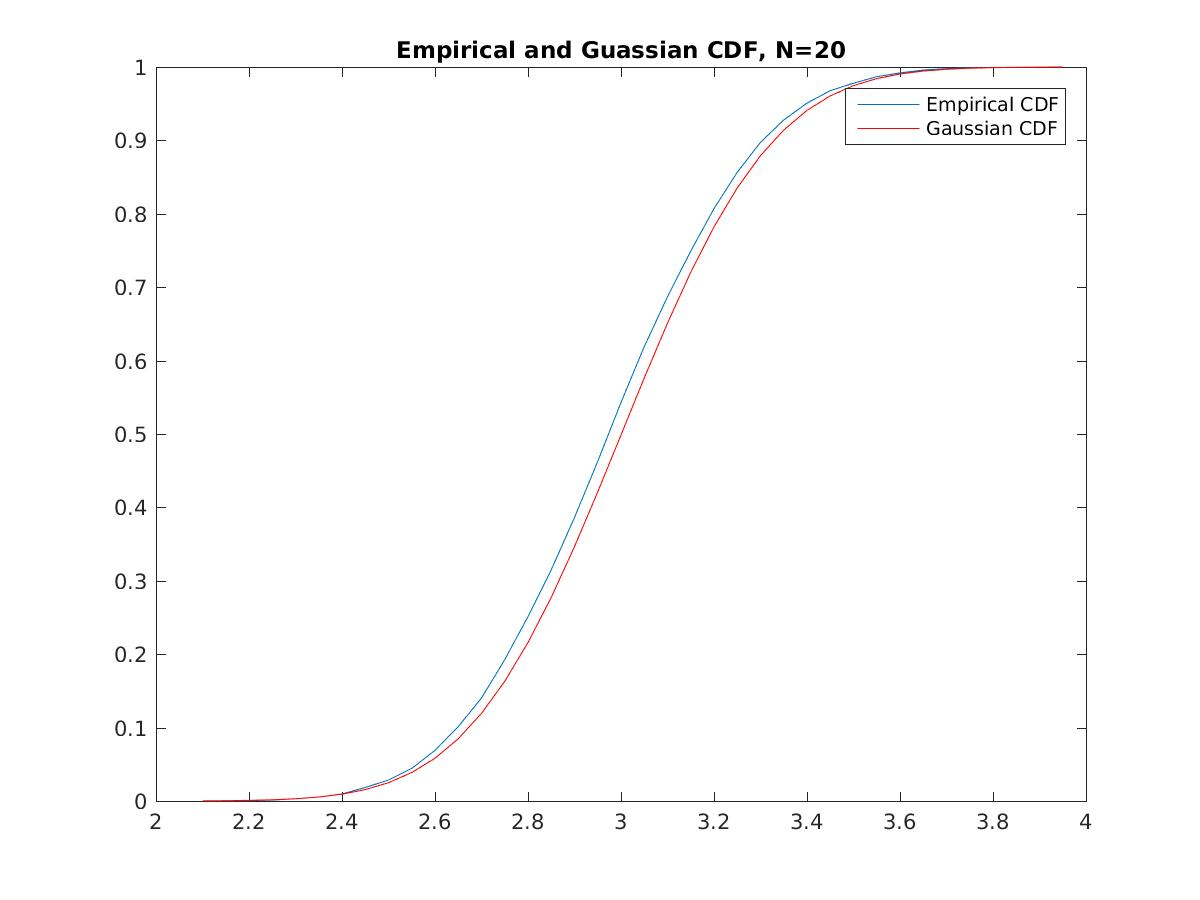
\includegraphics[width=\linewidth]{jpgs/cdfs/20_cdf.jpg}
    \caption{More Histogram.}
  \end{subfigure}
  \caption{N=20}
\end{figure}

\begin{figure}[h!]
  \centering
  \begin{subfigure}[b]{0.4\linewidth}
    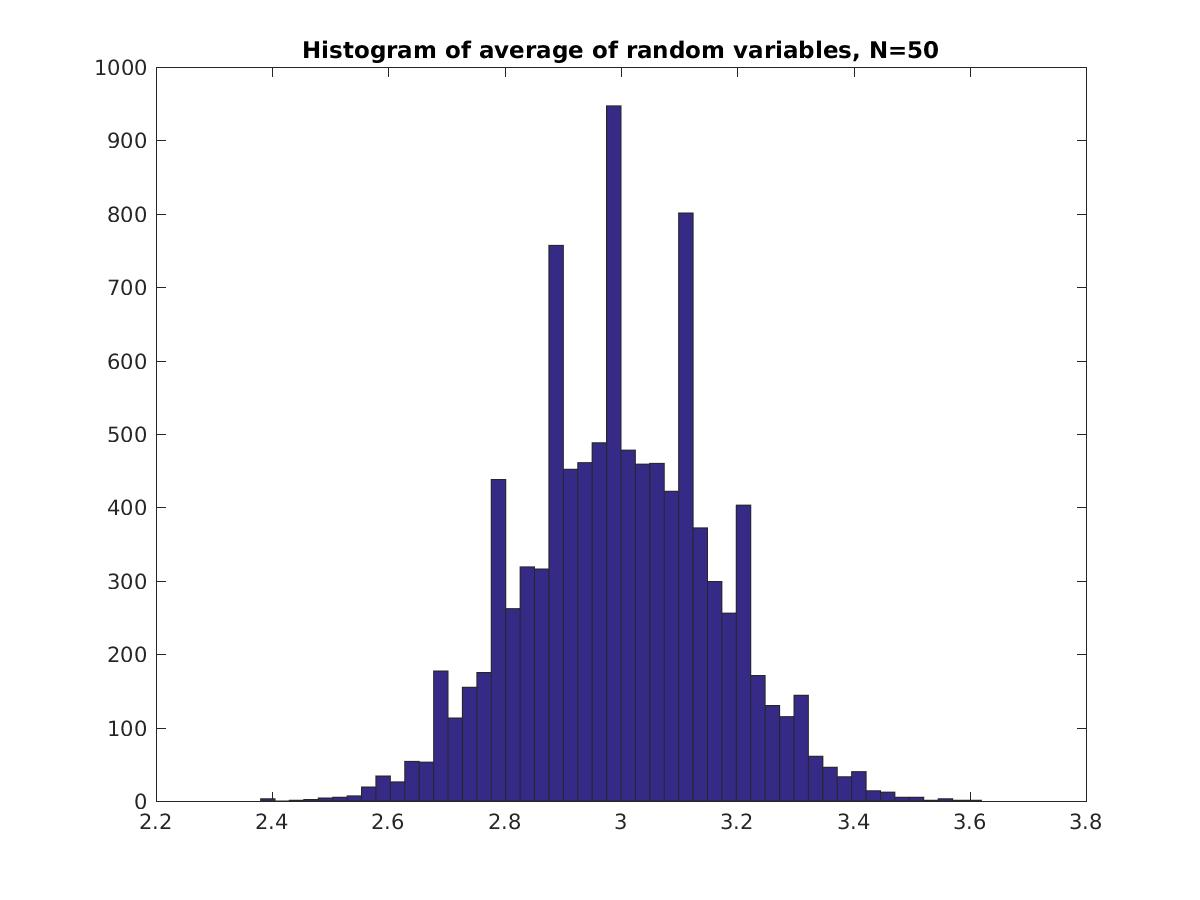
\includegraphics[width=\linewidth]{jpgs/histograms/50_hist.jpg}
    \caption{Histogram.}
  \end{subfigure}
  \begin{subfigure}[b]{0.4\linewidth}
    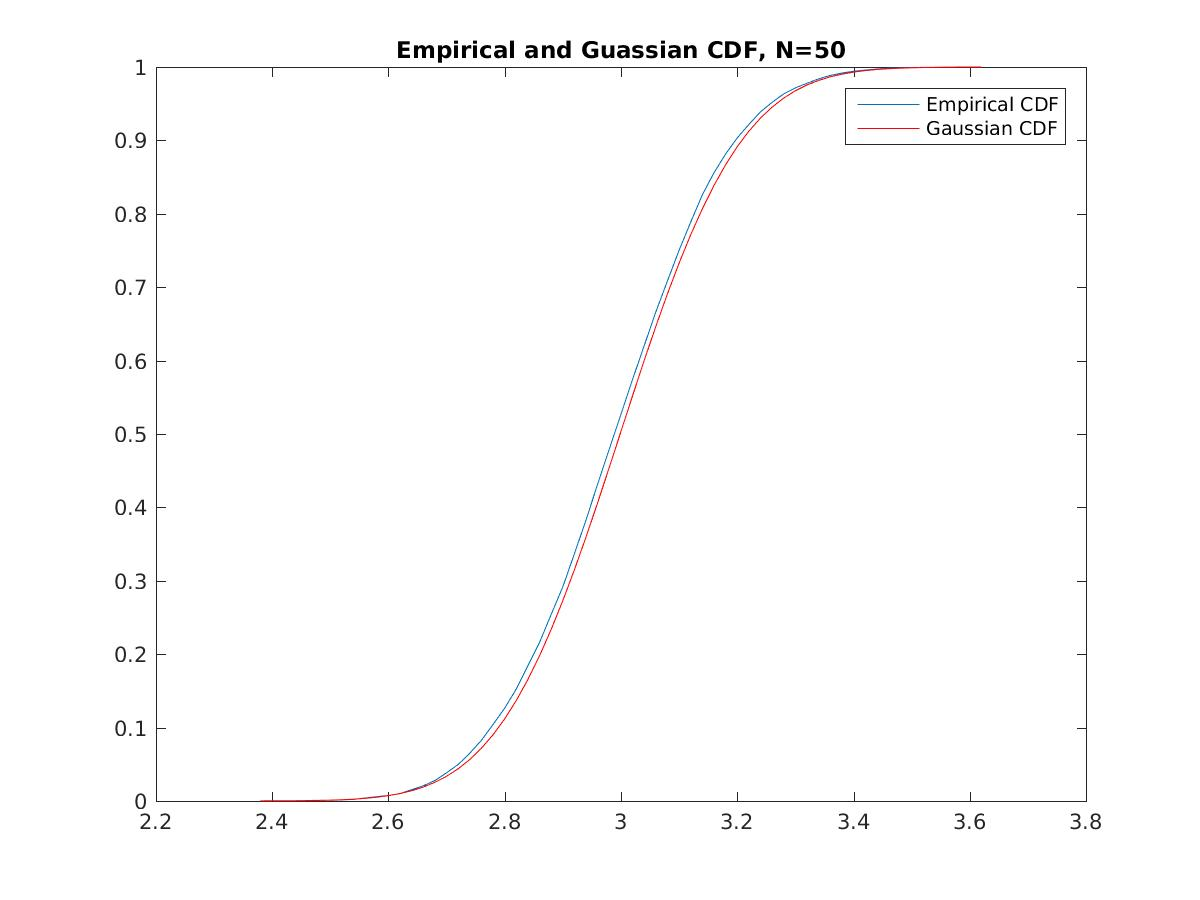
\includegraphics[width=\linewidth]{jpgs/cdfs/50_cdf.jpg}
    \caption{More Histogram.}
  \end{subfigure}
  \caption{N=50}
\end{figure}

\begin{figure}[h!]
  \centering
  \begin{subfigure}[b]{0.4\linewidth}
    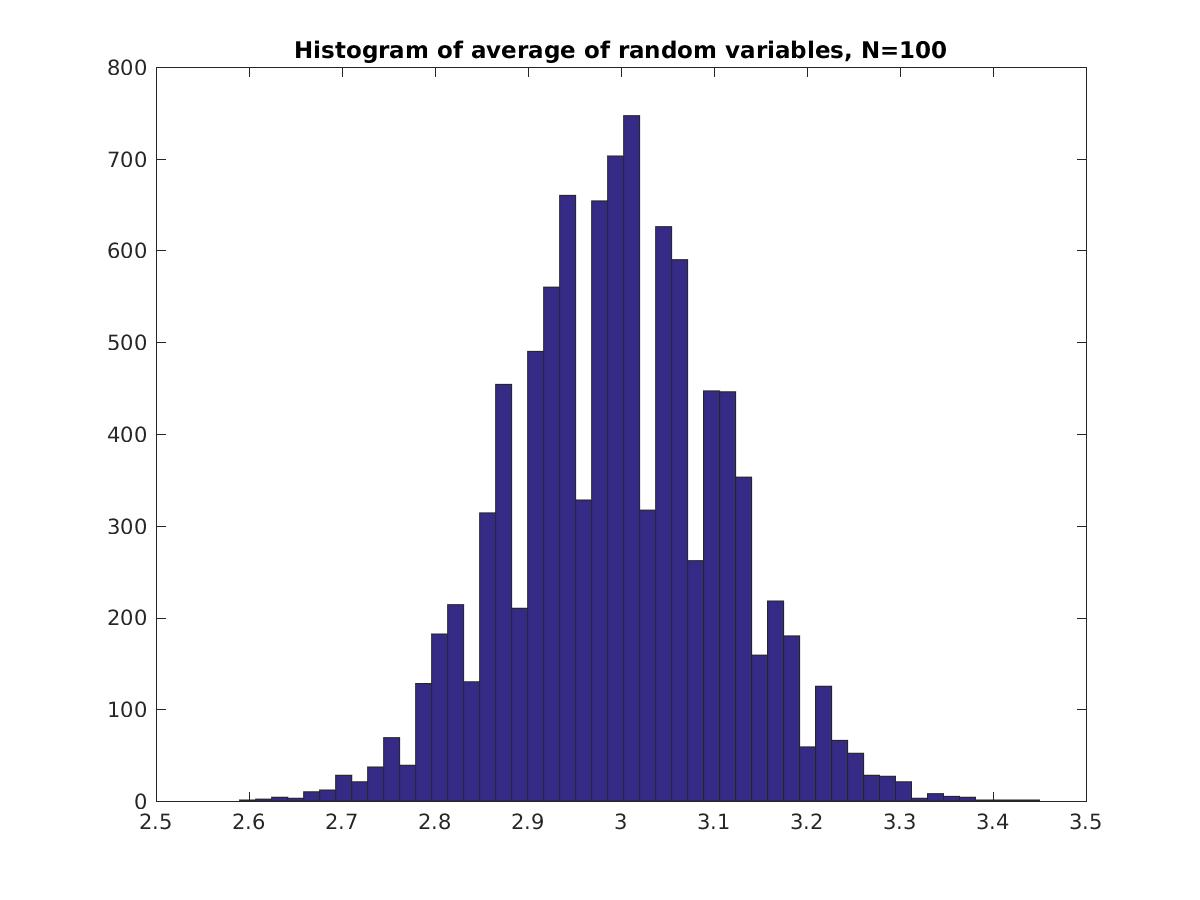
\includegraphics[width=\linewidth]{jpgs/histograms/100_hist.jpg}
    \caption{Histogram.}
  \end{subfigure}
  \begin{subfigure}[b]{0.4\linewidth}
    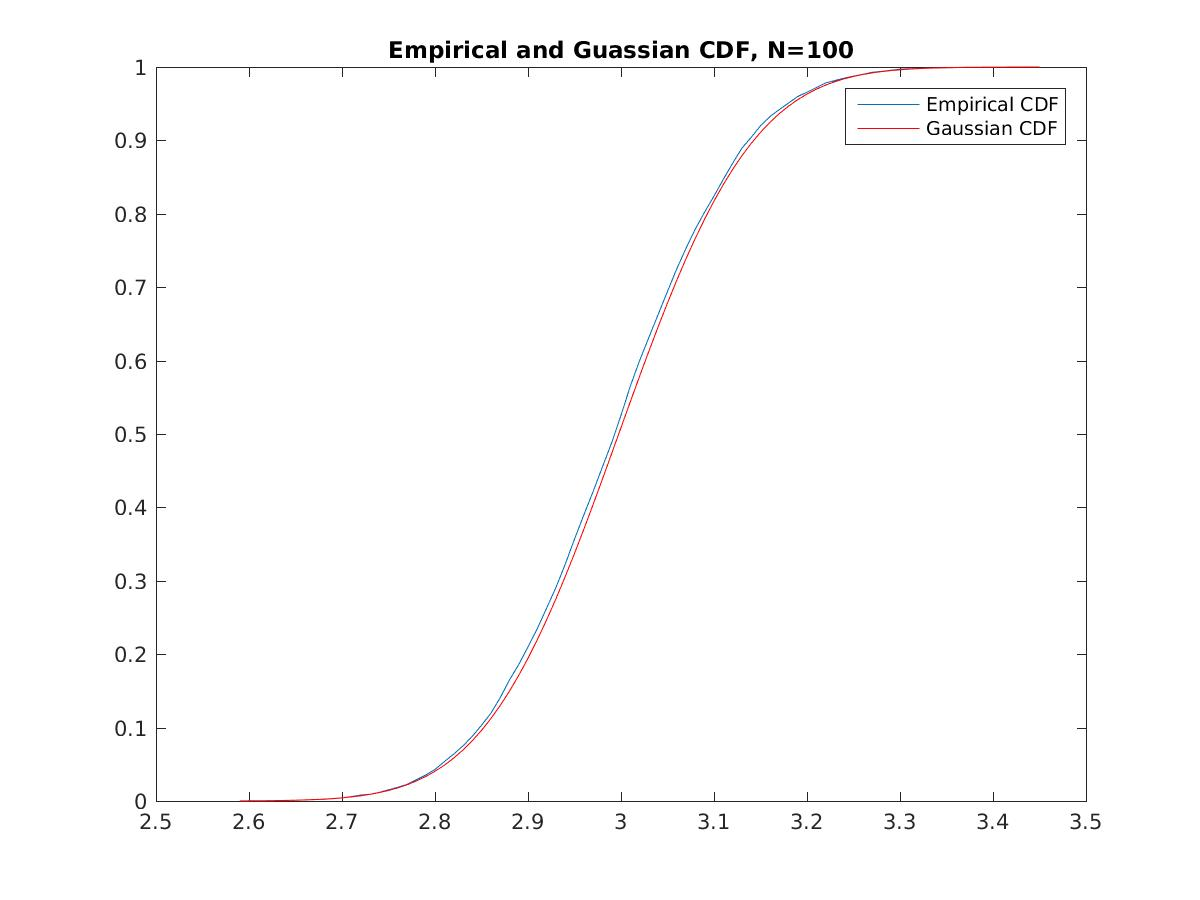
\includegraphics[width=\linewidth]{jpgs/cdfs/100_cdf.jpg}
    \caption{More Histogram.}
  \end{subfigure}
  \caption{N=100}
\end{figure}

\begin{figure}[h!]
  \centering
  \begin{subfigure}[b]{0.4\linewidth}
    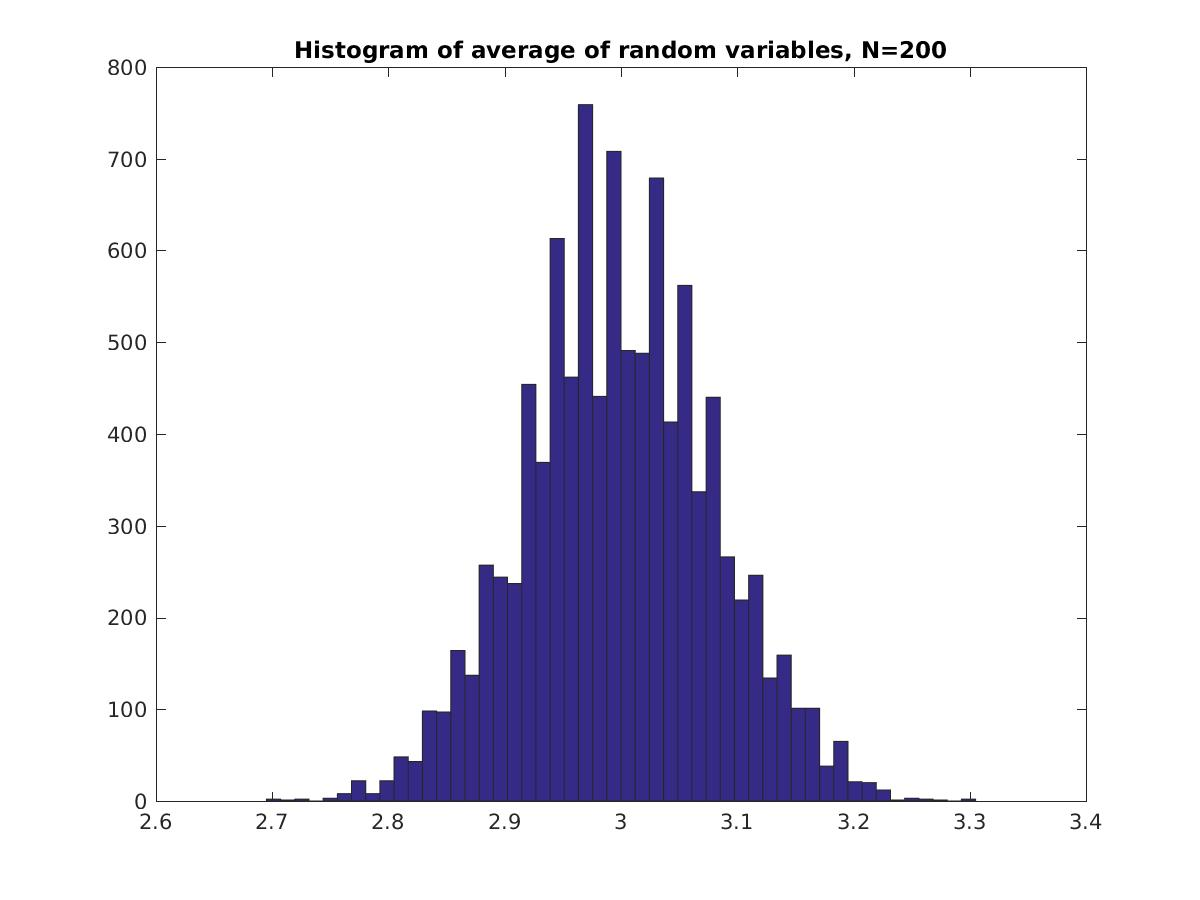
\includegraphics[width=\linewidth]{jpgs/histograms/200_hist.jpg}
    \caption{Histogram.}
  \end{subfigure}
  \begin{subfigure}[b]{0.4\linewidth}
    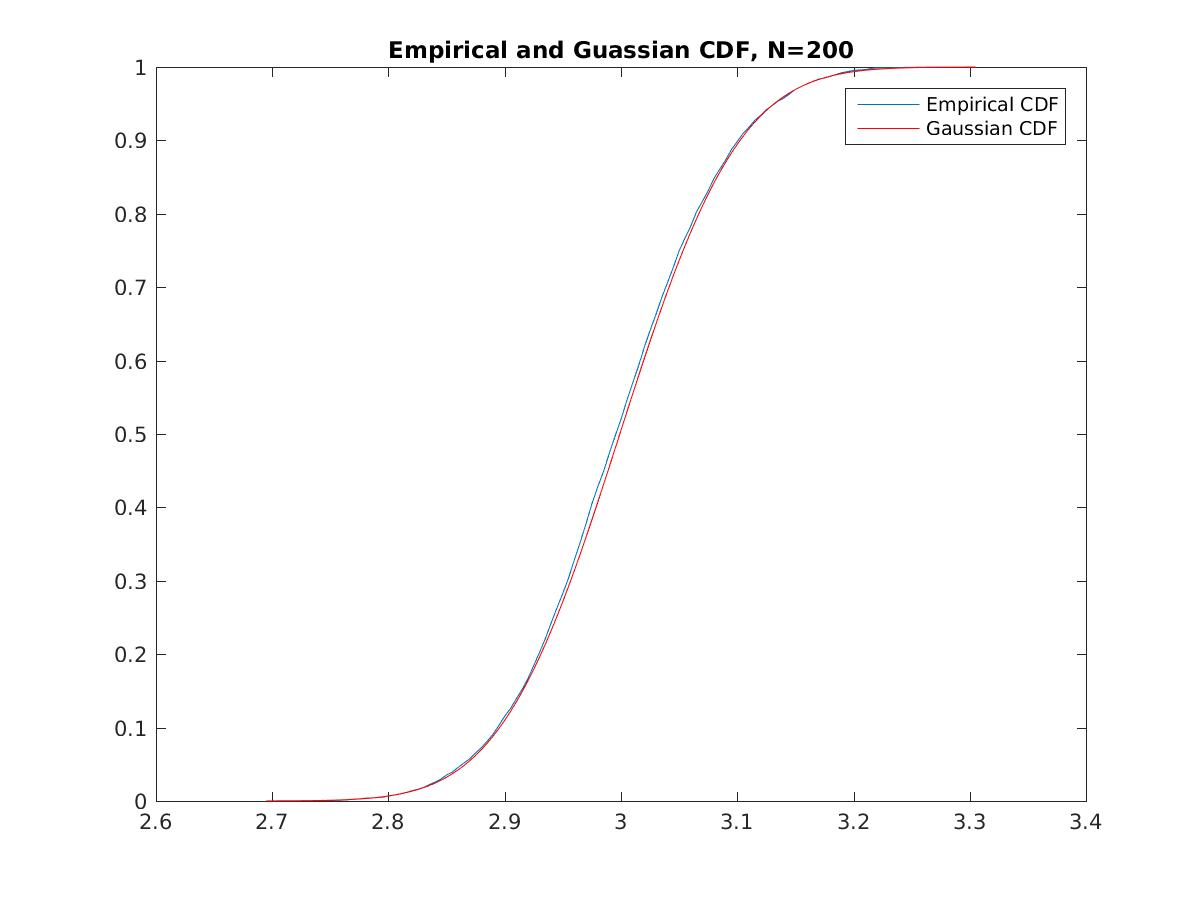
\includegraphics[width=\linewidth]{jpgs/cdfs/200_cdf.jpg}
    \caption{More Histogram.}
  \end{subfigure}
  \caption{N=200}
\end{figure}

\begin{figure}[h!]
  \centering
  \begin{subfigure}[b]{0.4\linewidth}
    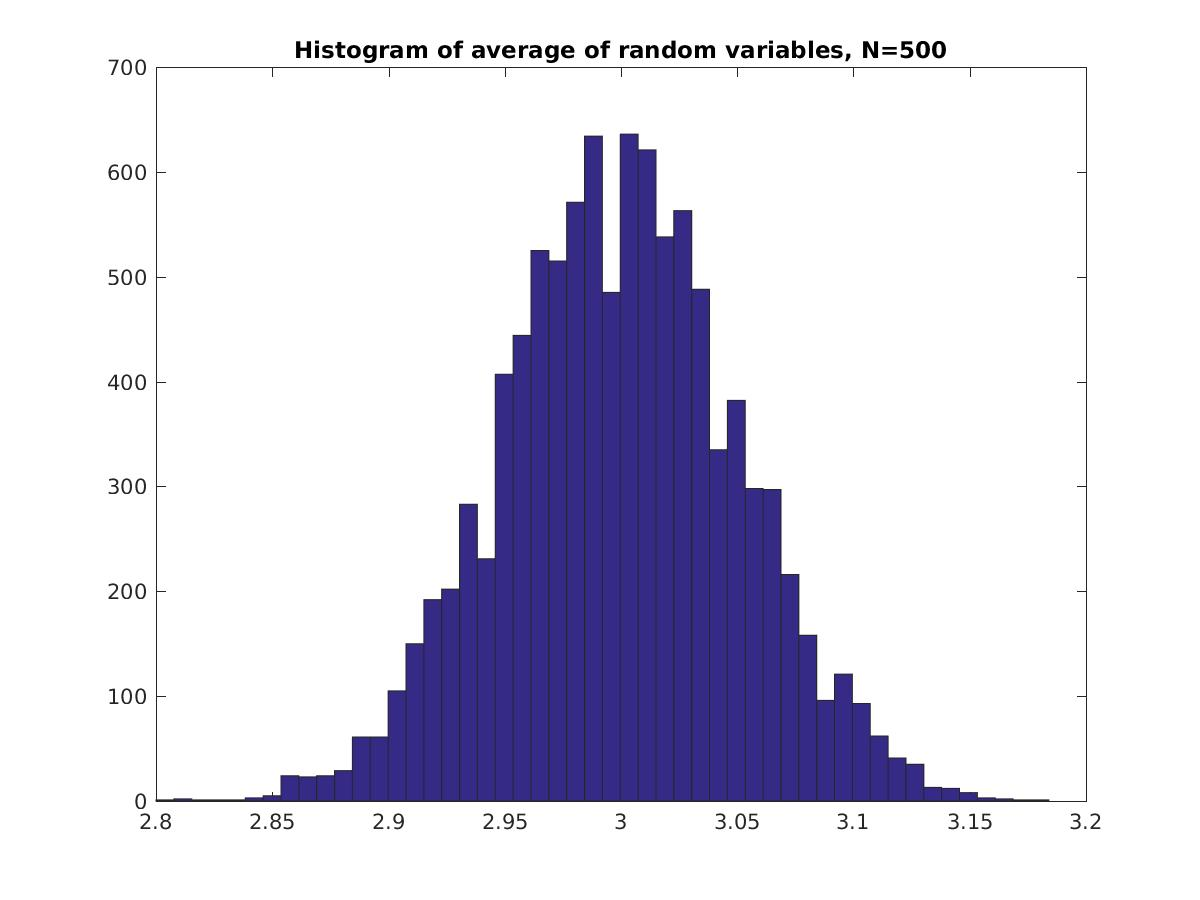
\includegraphics[width=\linewidth]{jpgs/histograms/500_hist.jpg}
    \caption{Histogram.}
  \end{subfigure}
  \begin{subfigure}[b]{0.4\linewidth}
    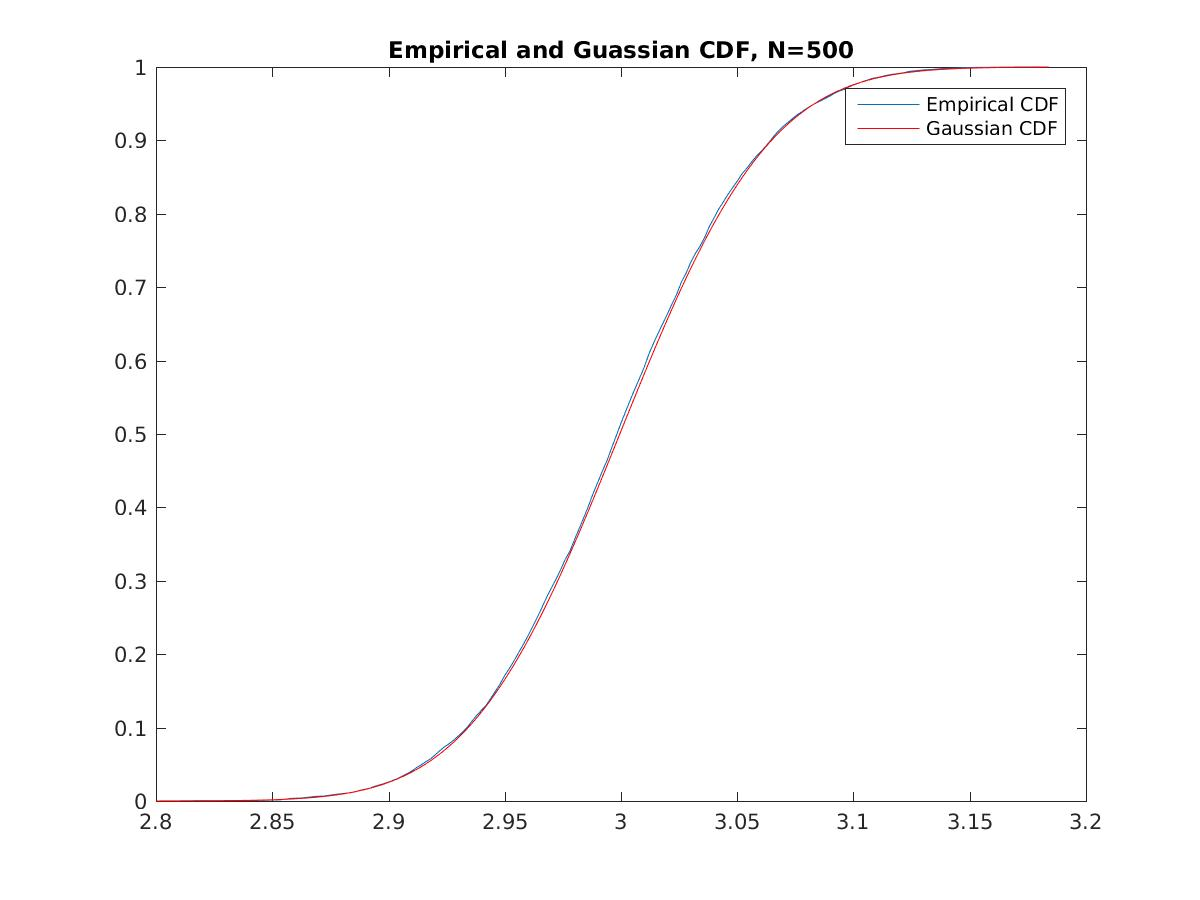
\includegraphics[width=\linewidth]{jpgs/cdfs/500_cdf.jpg}
    \caption{More Histogram.}
  \end{subfigure}
  \caption{N=500}
\end{figure}

\begin{figure}[h!]
  \centering
  \begin{subfigure}[b]{0.4\linewidth}
    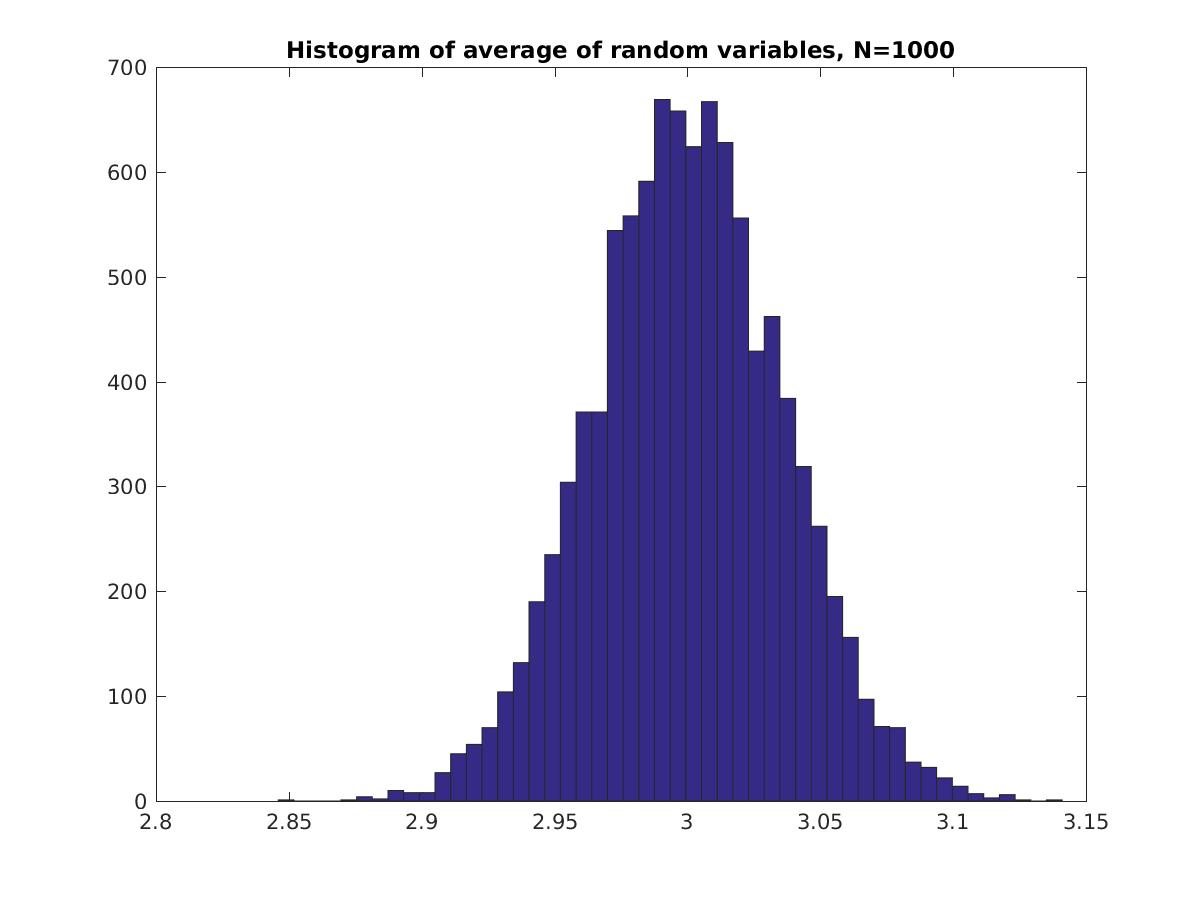
\includegraphics[width=\linewidth]{jpgs/histograms/1000_hist.jpg}
    \caption{Histogram.}
  \end{subfigure}
  \begin{subfigure}[b]{0.4\linewidth}
    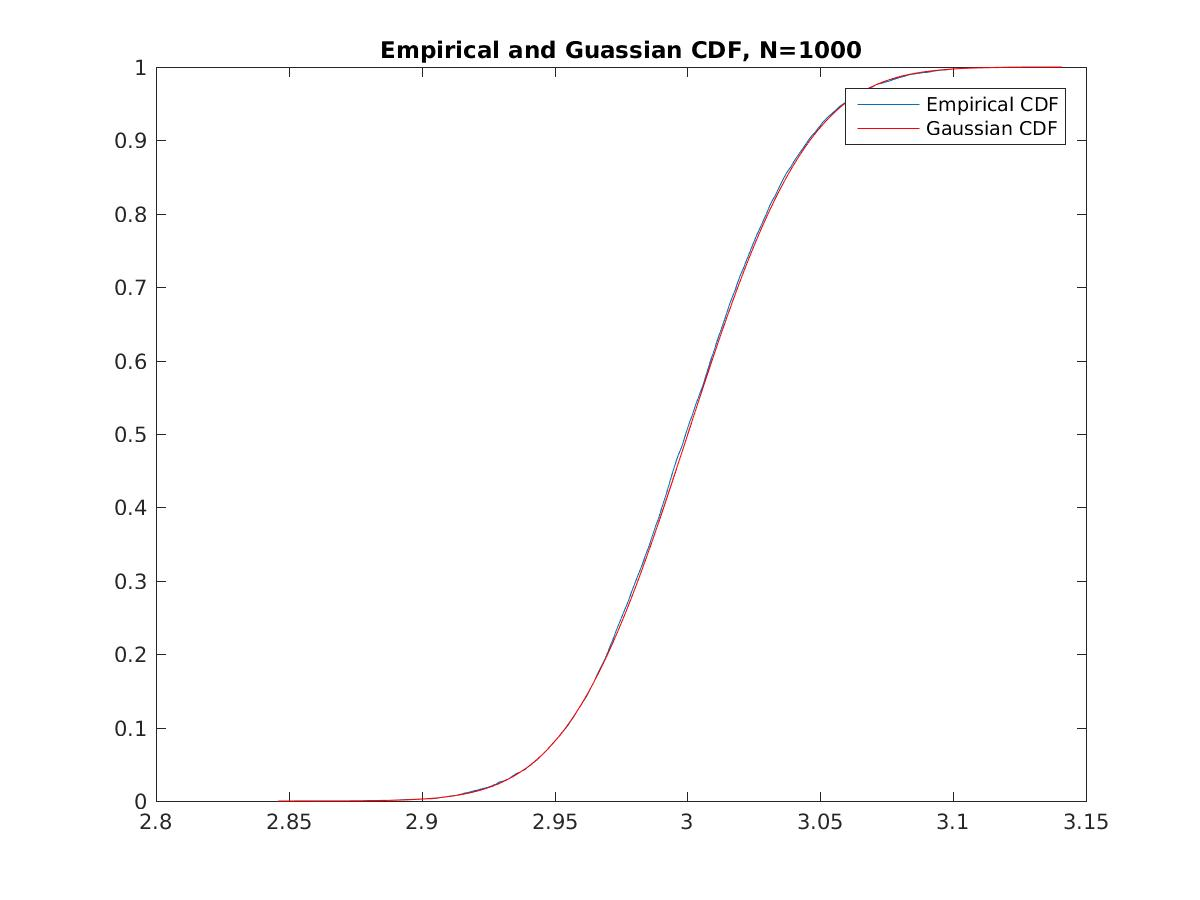
\includegraphics[width=\linewidth]{jpgs/cdfs/1000_cdf.jpg}
    \caption{CDF.}
  \end{subfigure}
  \caption{N=1000}
\end{figure}

\begin{figure}[h!]
  \centering
  \begin{subfigure}[b]{0.4\linewidth}
    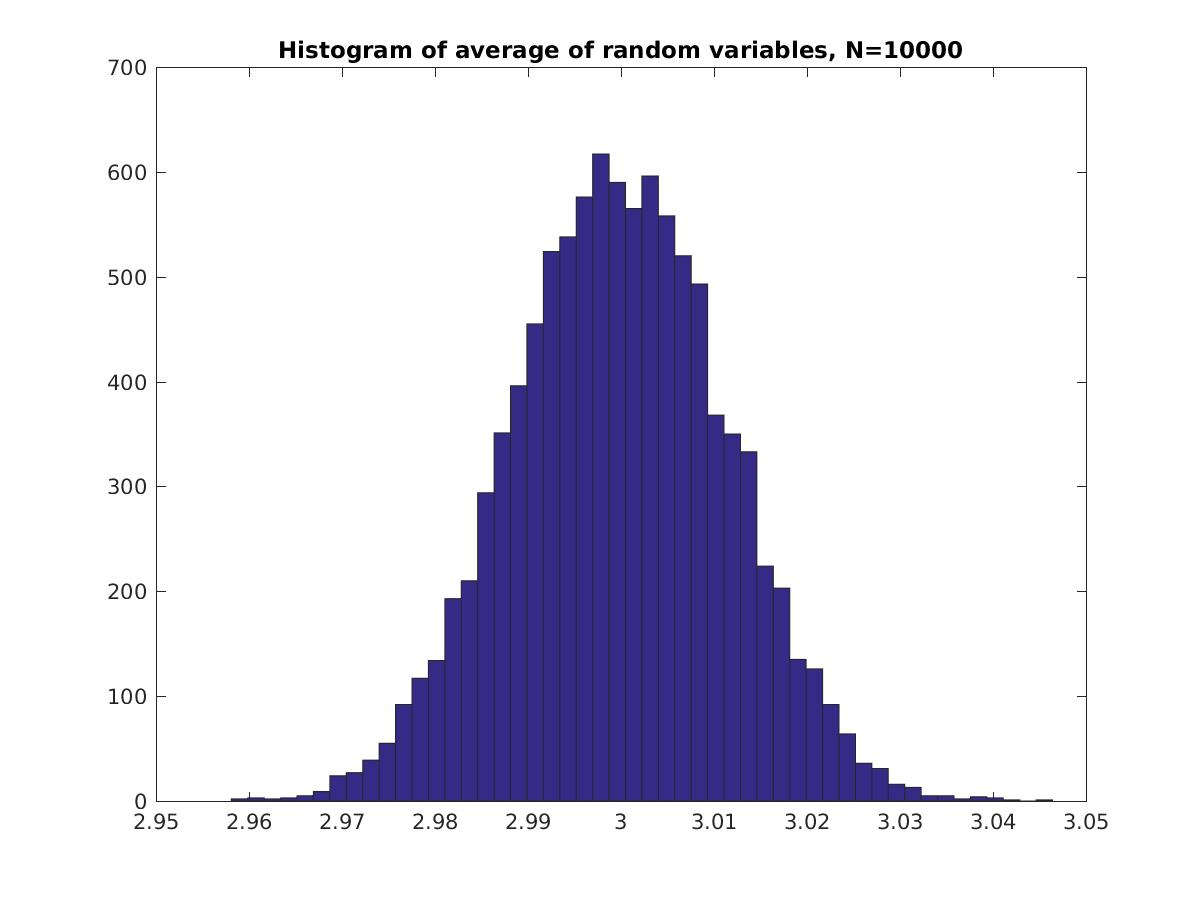
\includegraphics[width=\linewidth]{jpgs/histograms/10000_hist.jpg}
    \caption{Histogram.}
  \end{subfigure}
  \begin{subfigure}[b]{0.4\linewidth}
    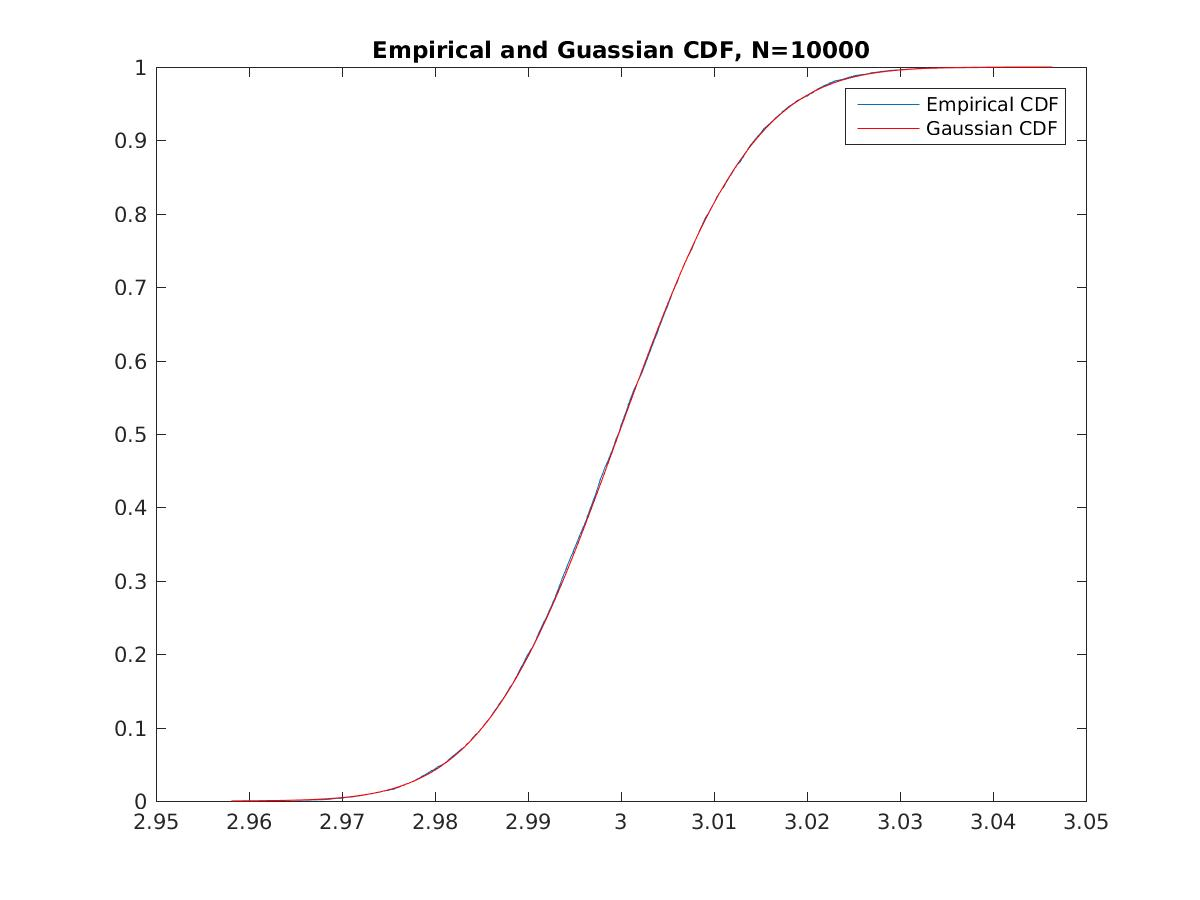
\includegraphics[width=\linewidth]{jpgs/cdfs/10000_cdf.jpg}
    \caption{CDF.}
  \end{subfigure}
  \caption{N=10000}
\end{figure}

\begin{figure}[h!]
  \centering
  \begin{subfigure}[b]{0.4\linewidth}
    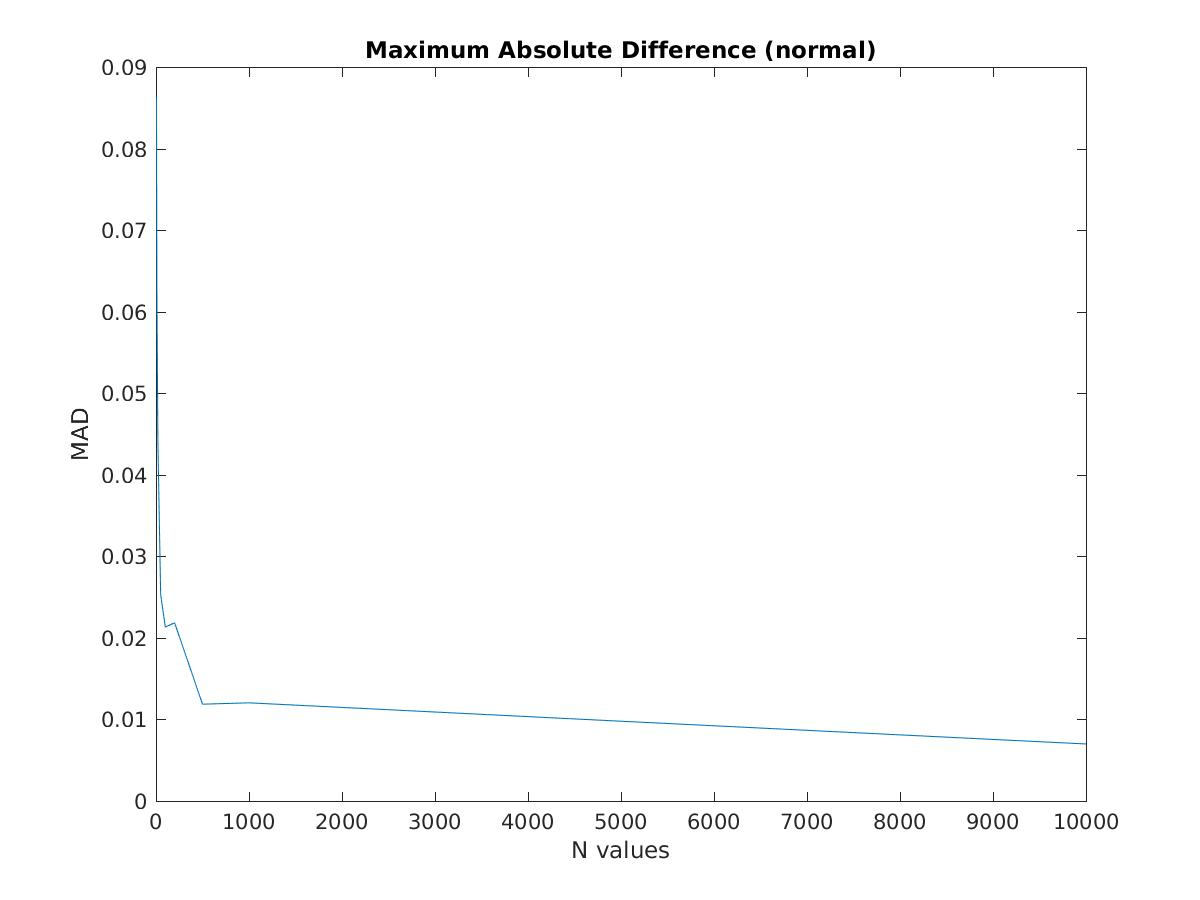
\includegraphics[width=\linewidth]{jpgs/mad.jpg}
    \caption{plotted against N}
  \end{subfigure}
  \begin{subfigure}[b]{0.4\linewidth}
    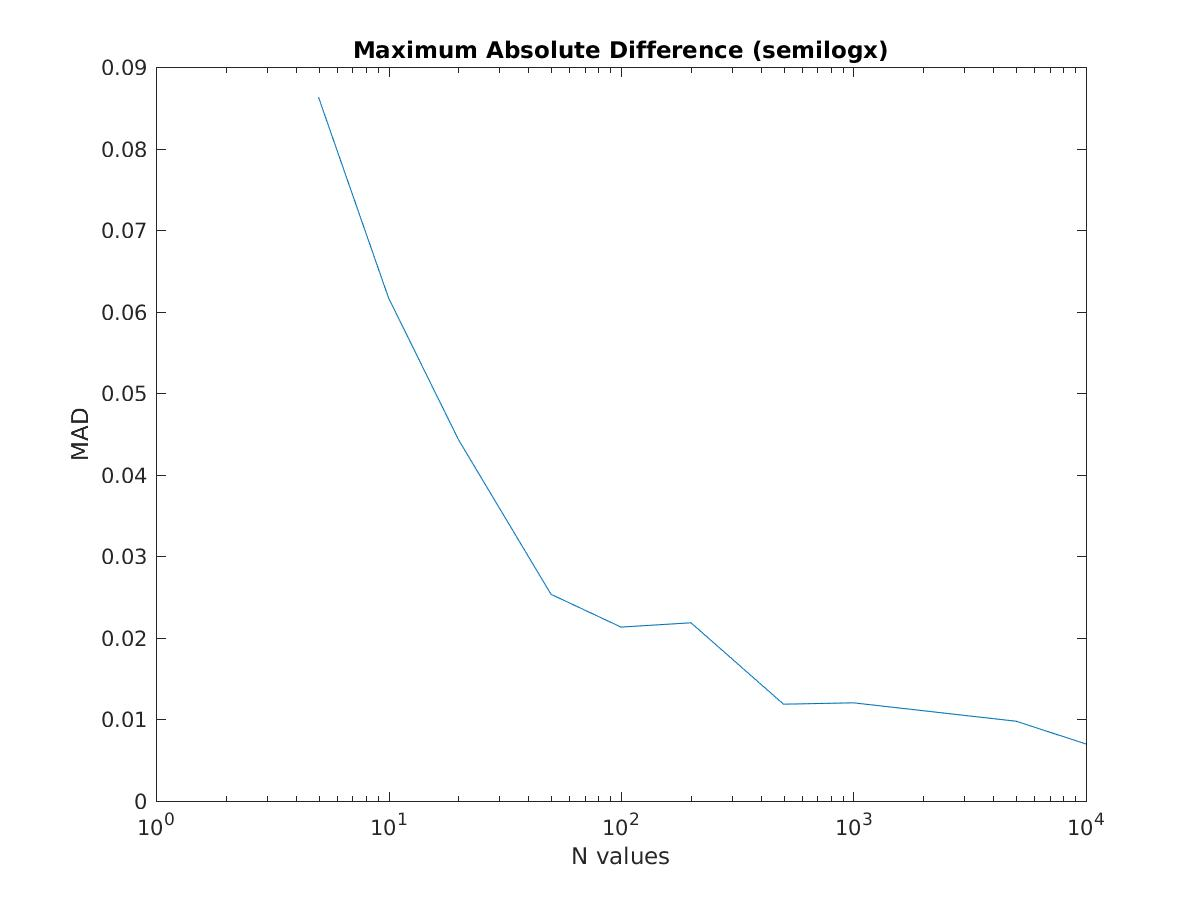
\includegraphics[width=\linewidth]{jpgs/mad_semilogx.jpg}
    \caption{plotted against semilogx(N)}
  \end{subfigure}
  \caption{MAD}
\end{figure}

As the value of N increases, the histogram starts resembling a bell curve
\newpage


\newpage
\section{Question 6}
\paragraph{Case I : Comparing Figure 1 and Figure 2\newline}
The figures given 'T1.jpg' and 'T2.jpg' were loaded in matlab. The second image was shifted by a range from -10 to 10, and the correlation coefficient, and QMI was calculated and plotted for every shift.
\begin{description}
\item[Correlation Coefficient] In the first case, we can observe that the plot of correlation coefficient achieves minimum at -1. By the defination, we can say that both the images are aligned 'the best' when the second image is shifted by -1. We can also conclude that the second image is apart by a pixel, as compared to the first image.
\item[QMI] The QMI is the squared summation of the difference between the joiont pdf and the product of the marginal pdfs. We can say that higher the values of the qmi, more will be the dependence between two images. In our plot, the best value of qmi is obtained when the shift is by -1, which supports our conclusion that the images are a pixel apart. We can also observe that the values of qmi are very low in the first case. This is because there is no 'explicit' relation between the two images.
\newline
\end{description}

\paragraph{Case II : Comparing Figure 1 and negative of Figure 1\newline}
The figures given 'T1.jpg' was loaded in matlab. The negative of the image was stored as another image and was shifted by a range from -10 to 10. The correlation coefficient, and QMI was calculated and plotted for every shift.
\begin{description}
\item[Correlation Coefficient] In this first case, we can observe that the plot of correlation coefficient achieves a perfect -1 at a shift of zero. This is because both the images are physically the same, with just negative intensities. So, at zero shift, they will have the most common part and the least correlation coefficient coefficient. As the image is shifter further, the images get more and more misaligned which lead in an increase in the correlation coefficient.
\item[QMI] In this case, since both the images are just the negative of one another, the peak of the qmi is achieved when the shift is zero. Also, we can see that this qmi plot falls off faster than the one observed in the first case. This is because when we shift by, say tx, then the first tx columns are completely reduced to 0. 
\end{description}

\paragraph{Usage of MATLAB Code}
\begin{itemize}
\item Load code in the following path 'matlab\_code/Q6/q6.m'
\item Run the code.
\item This will create 4 different plots for - Correlation coefficient, QMI, and both of these again when we compare with the first image with it's negative. 
\item These plots have been included in the report, as well as can be found in the directory 'matlab\_code/Q6/jpgs'
\end{itemize}


\begin{figure} [h!]
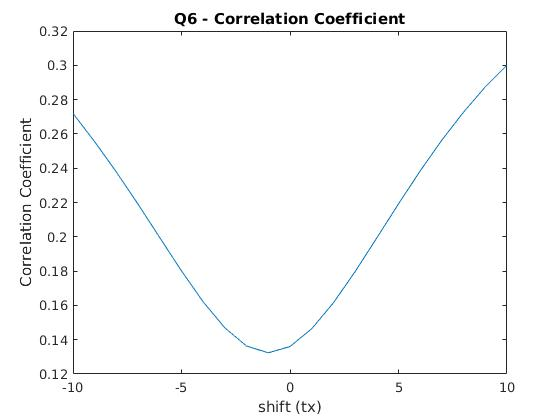
\includegraphics[width=\linewidth]{corr.jpg}
\caption{}
\label{fig:6.1}
\end{figure}

\begin{figure}[h!]
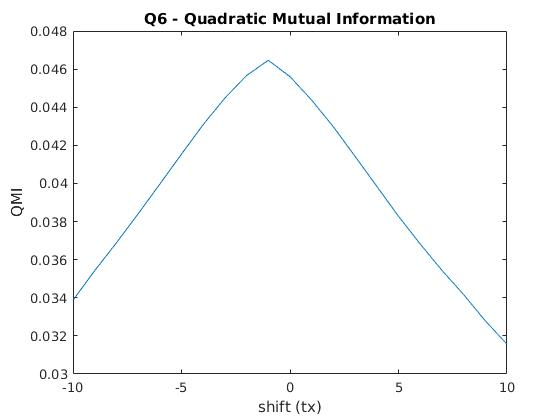
\includegraphics[width=\linewidth]{qmi.jpg}
\caption{}
\label{fig:6.2}
\end{figure}

\begin{figure} [h!]
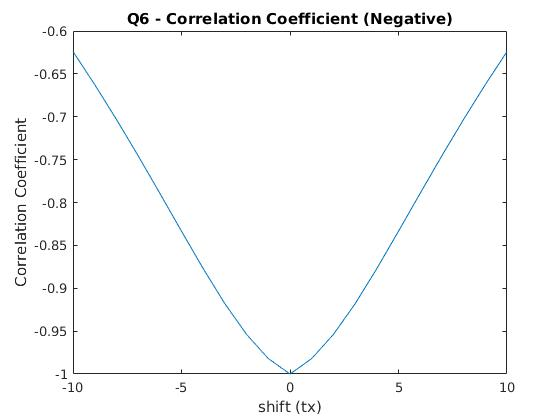
\includegraphics[width=\linewidth]{corr_neg.jpg}
\caption{}
\label{fig:6.3}
\end{figure}

\begin{figure} [h!]
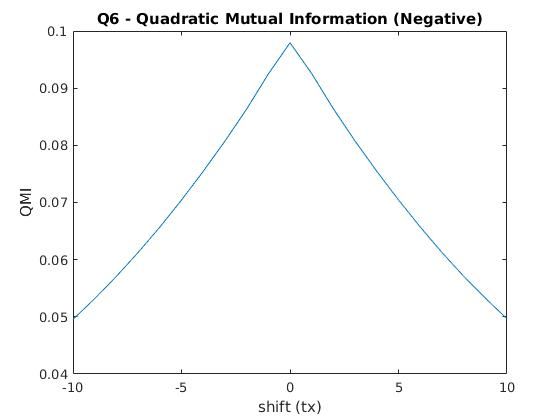
\includegraphics[width=\linewidth]{qmi_neg.jpg}
\caption{}
\label{fig:6.4}
\end{figure}


\end{document}